% =====================================================================
% Systematic Uncertainties
% H1 high-Q^2 charged-particle SIDIS analysis note
% =====================================================================
\section{Systematic Uncertainties}
\label{sec:systematics}

The current high-$\Qsq$ analysis release has detector, unfolding,
tracking-efficiency, hadron-azimuth, luminosity, radiative, and
background-subtraction systematic components assembled on the validated
490-row release contract.  It uses the near-electron cone selection with the
detector-interaction-corrected response and the pre-unfold subtraction of the
electron, V0, and low-$\Qsq$ background templates; the iterative Bayesian
unfolding of the subtracted data vector is the single denominator for every
relative component.  The frozen 2026-10-19 edition is
\path{systematics_bgsub_env100_21comp_2026-10-19/} under
\path{H1ChargedSidis_HighQ2/output_v6/central/data_release/}.  It inventories
21 columns: 20 active quadrature terms and the retired audit-only
\texttt{bgsub\_stat\_rel} column.  The active total,
\texttt{total\_with\_env100\_rel}, has medians of $7.320288331169215\%$ for
$\hplus$ and $7.637124635311324\%$ for $\hminus$, maxima of
$73.65119705575378\%$ and $88.43670499154085\%$, and no bins above $100\%$.
The frozen input, median, integrated-effect, and no-bin-above-$100\%$ gates
all passed.  This edition had superseded the 2026-10-17 19-component
clean-denominator budget as the quoted systematic; the latter is retained as
historical provenance.  Both frozen editions were computed on the central
values that the 2026-10-20 OPT-A baseline promotion superseded
(Sec.~\ref{sec:results:z005-release}): they are superseded as a quoting
basis, are retained unchanged as provenance, and the budget is being
regenerated on the OPT-A nominal
(Sec.~\ref{sec:syst:budget-regeneration}); until the regenerated budget
passes review, no per-bin uncertainty and no uncertainty total is final.
Global covariance matrices constructed from the frozen 2026-10-19 budget are
described in Sec.~\ref{sec:syst:global-covariance}.  The
radiative correction $C_{\mathrm{rad}}$ is applied to the cross section at
Born level, with its uncertainty carried as the two systematic components
described in Sec.~\ref{sec:radiative_corrections} and listed in
Table~\ref{tab:syst:z005-components}.  The remaining open item for the
radiative correction is its application at the multiplicity level.

\subsection{Budget Regeneration on the OPT-A Nominal}
\label{sec:syst:budget-regeneration}

The systematic budget is being regenerated on the OPT-A nominal central
values (Sec.~\ref{sec:results:z005-release}).  Until the regenerated budget
passes review, no per-bin uncertainty and no uncertainty total of the frozen
editions may be quoted as final.  The regeneration and its companion open
items are:
\begin{itemize}
  \item the re-derivation of the affected components on the OPT-A nominal,
        together with the fix of the detector-interaction double count in
        the twenty-active-term total: the removal term enters the quadrature
        sum twice, an inflation proven exactly in three independent
        re-derivations, of at most about $1.71\times10^{-4}$ relative and
        never deflating, so the frozen totals are strictly conservative;
  \item the per-bin treatment of the 56 published bins whose OPT-A Born
        shift exceeds the per-bin background-envelope component of the
        frozen budget (largest ratio 2.58; no bin exceeds the frozen
        edition totals, with maximum ratios 0.86 and 0.70 against the
        nineteen- and twenty-active-term editions, a statement robust to
        the double-count fix), and the assignment of a systematic home to
        the residual straddle-rate model dependence---the residual mismatch
        of the per-cell straddle rates between simulation and data, bounded
        by the same straddle logic;
  \item the form of the declared $z$-bin-row shift convention
        (Sec.~\ref{sec:unfolding:truth-contract}): caveat only, or a budget
        component; if a component is chosen, the only sound derivation is a
        self-consistent scheme pair---a response variant with the rad-safe
        generator $z$ together with a co-derived correction on the same
        basis---and never a rad-safe-$z$ response combined with the current
        correction table, which would double-count the $z$ migration;
  \item the reconstruction of the frozen-edition budget builder, whose
        provenance could not be located; the acceptance condition is the
        exact reproduction of the nineteen-component total on the three
        empty-subtracted-data bins (positive charge, bins 109 and 179;
        negative charge, bin 240);
  \item the missing HFS--$E-p_z$ systematic channel: the
        hadronic-final-state shifts leave $E-p_z$ bit-identical, so the
        quoted HFS-leg errors do not cover the $E-p_z>45~\GeV$ requirement;
  \item the re-basing of the fractional covariance product of
        Sec.~\ref{sec:syst:global-covariance} to the OPT-A nominal;
  \item the re-pointing and repair of the registered canonical plotting
        chain, whose script audit failed with 24 defects and whose
        registered Born plotter still reads a superseded release, and the
        remaining publication-facing canonical plot categories, which
        depend on the regenerated budget.
\end{itemize}

\subsection{List of Systematics}
\label{sec:syst:z005-components}

Table~\ref{tab:syst:z005-components} lists the components of the total
uncertainty as combined in the frozen budget editions
(Sec.~\ref{sec:syst:budget-regeneration}). The HFS and electron sources of uncertainty are calculated using the standard H1CalcSystematic framework.

\begin{table}[h]
\centering
\small
\begin{tabular}{p{4.5cm}p{10.3cm}}
\toprule
Component & Treatment \\
\midrule
IBU statistical uncertainty & $\sigma$ of 1000 Poisson-only toy replicas on the subtracted data vector \\
IBU model uncertainty & Difference in unfolded data with different model migration matrices \\
IBU regularization uncertainty & $\pm1$ iteration around nominal $N_{\mathrm{iter}}=4$ \\
Hadron-azimuth prior & Flat-$\phih$ IBU prior; half the larger generator deviation \\
Scattered-electron energy & 1\% shift of $E_{e'}$ \\
Scattered-electron polar angle & Shift of $\theta_{e'}$ by $1~\mathrm{mrad}$\\
Tracking efficiency & $-0.5\%$ tracking-efficiency shift\\
HFS JES & Shift of JES by 2\% \\
HFS RCES & Shift of RCES by 2\%\\
HFS polar angle & Shift of HFS $\theta$ by 1 mrad \\
Radiative generator difference & DJANGOH vs RAPGAP, median $0.5844/0.5804\%$ ($\hplus/\hminus$) \\
Radiative correction statistics & Statistical uncertainty, median $0.4272/0.4429\%$ ($\hplus/\hminus$) \\
Detector-integration removal & Removal-increment isolation of the detector-interaction reroute on the subtracted chain; median $0.0299/0.0287\%$ ($\hplus/\hminus$) \\
Fake-column MC statistics & Cone fake-column $\sigma(f_i)$ propagated through the unfolding Jacobian on the subtracted data vector; median $0.3437/0.3494\%$ ($\hplus/\hminus$) \\
Background-subtraction model & V0 and electron generator half-spreads in quadrature with a $\pm30\%$ low-$\Qsq$ scale term \\
Background-subtraction stage & Pre-versus-post-unfold stage difference measured on the cone chain \\
Background-subtraction fake fraction & Fake-fraction common-model dependence $|1-r_{\min}|\,f_i$ with the proxy $r_{\min}=0.9817$ (NucliaWeight caveat) \\
Background-subtraction envelope & Fully correlated $\pm100\%$ normalization envelope on $(e_{\mathrm{avg}}+V0_{\mathrm{avg}})/\mathrm{data}_{\mathrm{sub}}'$; \texttt{bgsub\_stat\_rel} is retained audit-only and excluded from the total \\
Luminosity & flat $2.7\%$ \\
\bottomrule
\end{tabular}
\caption{The systematic-uncertainty components of the frozen budget editions and how they are calculated.  The detector-integration removal entry comprises two terms, its model and statistical parts, so the inventory holds twenty active quadrature terms in total.  The audit-only retired \texttt{bgsub\_stat\_rel} column is not included in the quadrature sum.}
\label{tab:syst:z005-components}
\end{table}

The five detector components (scattered-electron energy and polar angle, and
HFS JES, RCES, and polar angle) are full-chain single-sided variations: the
shift is applied at the reconstructed electron or HFS and propagated through
the shifted-chain response and unfolding, with RAPGAP31 governing and absolute
single-sided differences taken; on the current background-subtracted release
the background templates are subtracted from each shifted data vector as
well.  For the
scattered-electron energy component
the leg with the larger robust median is used per charge, the leg-level
envelope; the HFS legs are produced in the plus direction only and their sign
symmetry is assumed, a deferred follow-up.  The tracking-efficiency component
remains a data-side conservative shift, with medians $0.5132\%$
($\hplus$) and $0.5211\%$ ($\hminus$) on the background-subtracted denominator.  The
two radiative components are unchanged by the detector-interaction,
cone-baseline, and background-subtraction promotions of the observable basis,
carried bit-identically.

The shifts applied to the HFS primarily enter the measurement through the calculation of $E-P_z$. They do not affect the tracks.

The electron and V0 background templates used in the pre-unfold subtraction
are MC-derived and their normalization
could not be measured by the dedicated control-region fits: in the
$|\mathrm{DcaPrime}|>0.25~\mathrm{cm}$ tail, the two-class model is
unidentifiable, with the V0 normalization at its lower bound and the electron
normalization drifting to $2.5$--$3.5$ in the failed groups, while five of the
eight fits fail and the accepted groups remain compatible with unity.  The
nominal subtraction corresponds to $7.28\%$ of the cone data vector, composed
of $3.85\%$ electron and $3.42\%$ V0 content; it is therefore assigned the
fully correlated $\pm100\%$ envelope
$\texttt{bgsub\_env100\_rel}=(e_{\mathrm{avg}}+V0_{\mathrm{avg}})/\mathrm{data}_{\mathrm{sub}}'$
rather than using the retired template-statistics term.  The tightened-chain
check, in which $|\mathrm{DcaPrime}|<0.3~\mathrm{cm}$ is propagated through
data, response, templates, and unfolding, finds 87 shifts above $3\sigma$
where 1.21 are expected from statistical fluctuations; its integrated Born
changes, $-2.37\%$ ($\hplus$) and $-1.40\%$ ($\hminus$), require correlated
content uncertainties of $30.7\%$ and $17.6\%$, respectively.  In the
per-bin requirement study, 23 significant shifts require more than $30\%$,
10 require more than $50\%$, and the largest requirement is $97\%$; every
significant shift is contained by the $\pm100\%$ envelope.  The earlier DCA
scan is a diagnostic-only far-tail study, not a component of the quoted
budget; crediting even its one-sided tightening does not remove the need for
the envelope.  The DCA removal itself rejects $200\%$--$300\%$ more tracks
than the associated template background, so the residual tail excess is of
unknown composition and can include displaced signal.  The residual risk is
therefore recorded rather than interpreted as a background measurement: the
coherent envelope is $7.715610295533167\%$ ($\hplus$) and
$7.973016448067494\%$ ($\hminus$), corresponding at Born level to
$\pm0.9256076766034321~\mathrm{nb}$ and
$\pm0.929969093275612~\mathrm{nb}$ on the $11.996558161307064~\mathrm{nb}$
and $11.663955534683723~\mathrm{nb}$ integrated cross sections, respectively.
The fully correlated treatment is retained across bins and charges.  It does
not remove the standing caveats on the low-$\Qsq$ template scale, the
NucliaWeight fake-fraction proxy, or the blocked DIFFVM and photoproduction
register rows; the near-electron cone remains motivated by the previous H1
charged-particle measurement~\cite{H1:2013qsm}.

\subsection{Per-Source Fractional-Uncertainties}
\label{sec:syst:source-plots}

Figures~\ref{fig:syst:sources-hplus-env100-fullrange}--\ref{fig:syst:sources-hminus-env100-midrange}
display the per-source fractional systematic uncertainties and their quadrature
sum for $\hplus$ and $\hminus$ in percent units.  The display shows all 21
inventory components, the active total, and the superseded 19-component total
as a dashed reference.  The active total is
\texttt{total\_with\_env100\_rel}, with medians $7.320288331169215\%$ for
$\hplus$ and $7.637124635311324\%$ for $\hminus$.  The retired audit-only
\texttt{bgsub\_stat\_rel}
column is not plotted or included in this total.

The three fixed vertical ranges provide the full 0--100\% range, the 0--15\%
zoom, and the intermediate 0--50\% range.  The figures are dated
candidate renderings of the frozen 2026-10-19 budget, which is superseded as
a quoting basis (Sec.~\ref{sec:syst:budget-regeneration}); the
publication-version plotting script for these panels is not yet registered.

\begin{figure}[p]
  \centering
  \begin{subfigure}[t]{0.98\textwidth}
    \centering
    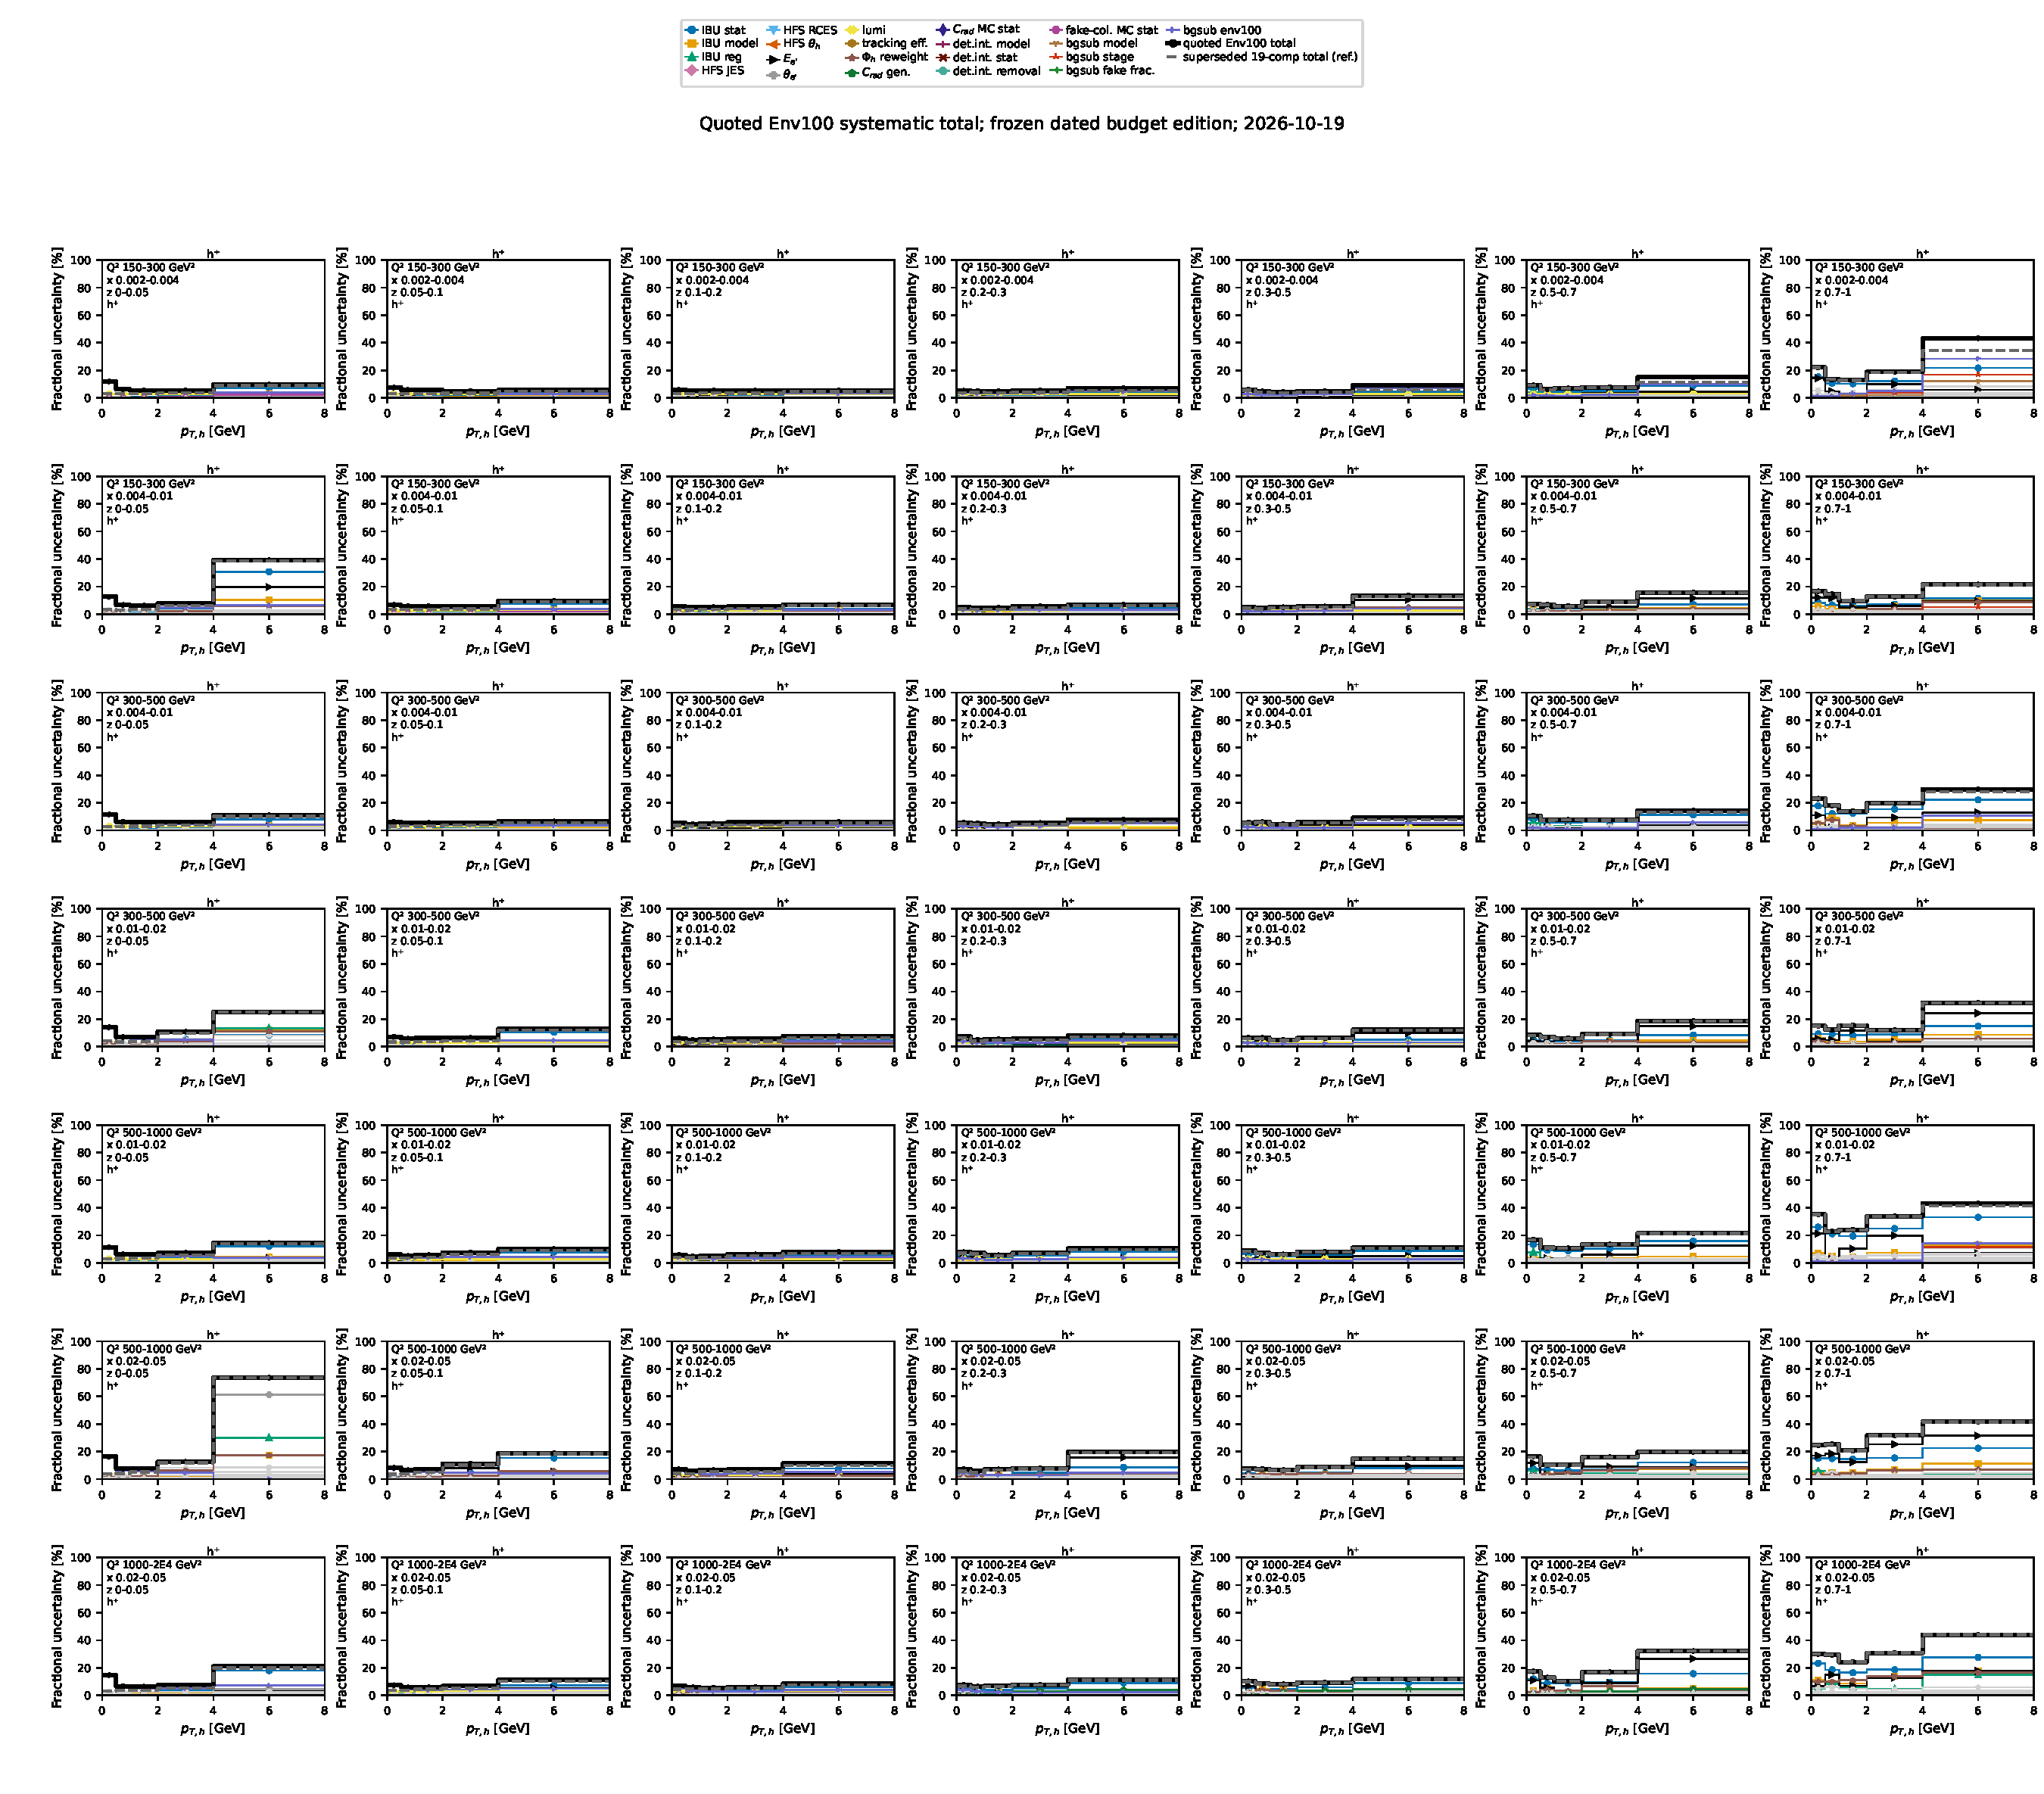
\includegraphics[width=\textwidth,height=0.38\textheight,keepaspectratio]{figures/fig_syst_uncertainty_sources_hplus_env100_ylim100.pdf}
    \caption{Full 0--100\% range.}
  \end{subfigure}
  \par\medskip
  \begin{subfigure}[t]{0.98\textwidth}
    \centering
    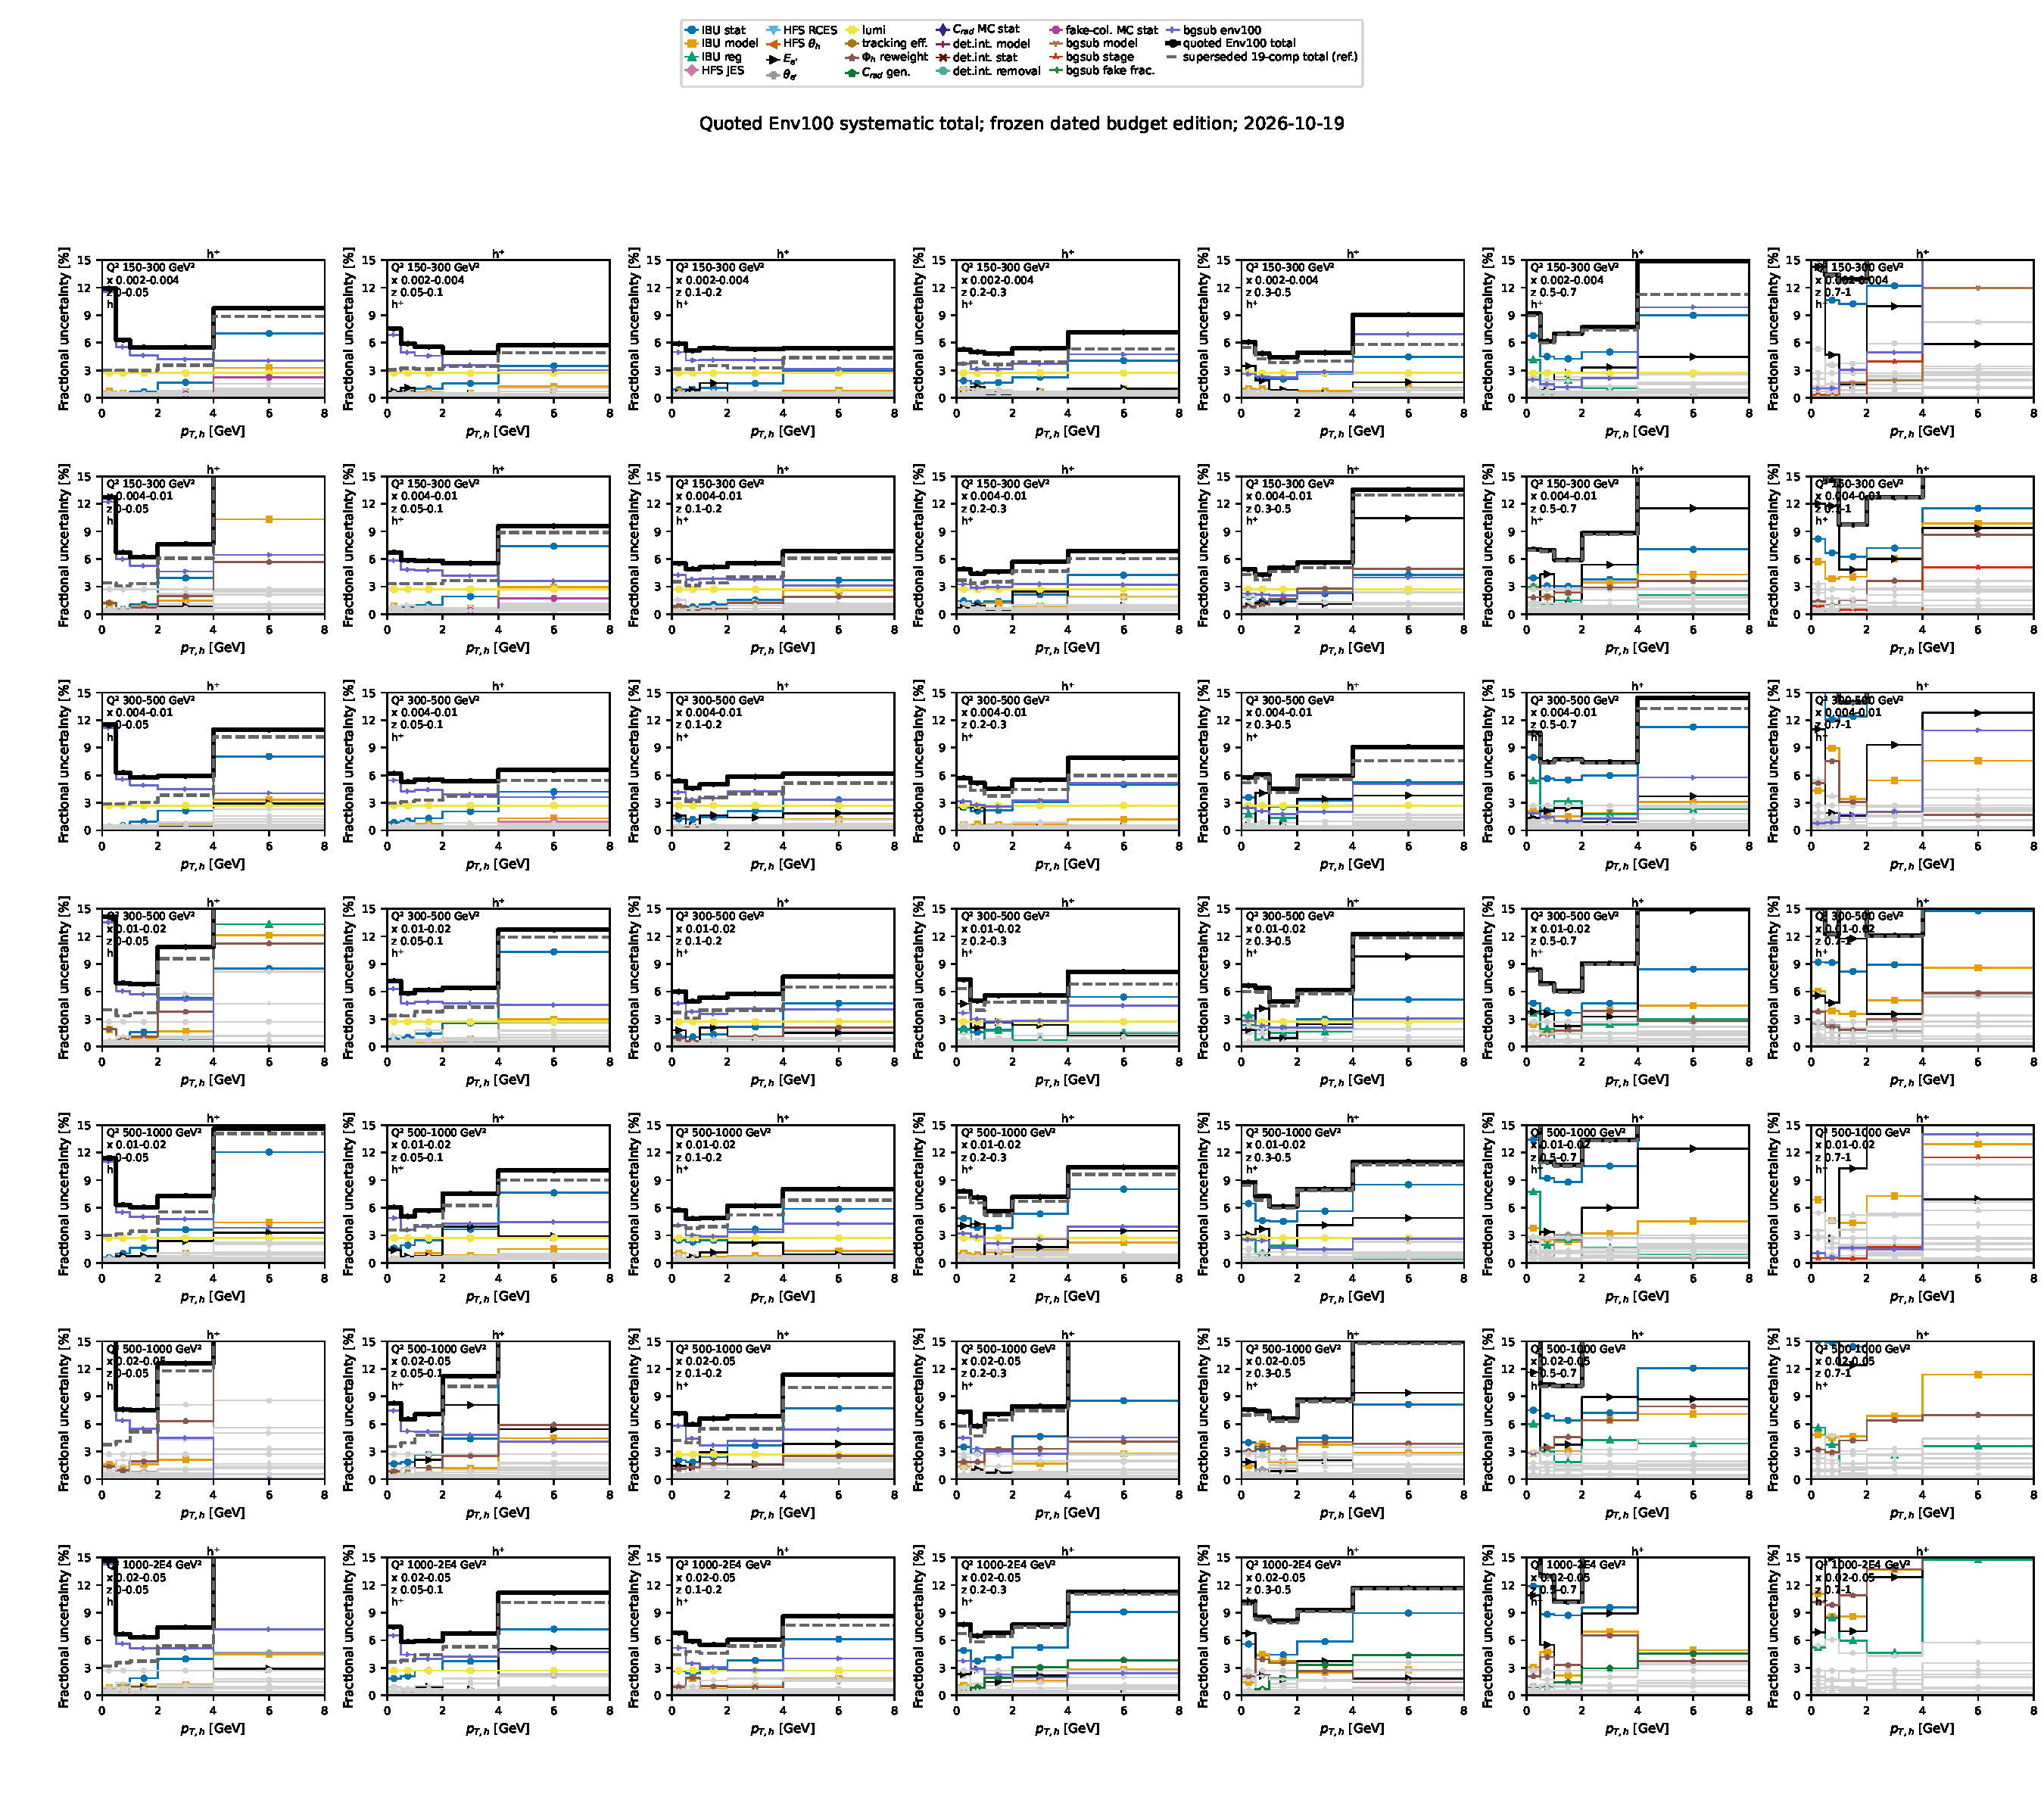
\includegraphics[width=\textwidth,height=0.38\textheight,keepaspectratio]{figures/fig_syst_uncertainty_sources_hplus_env100_ylim015.pdf}
    \caption{0--15\% zoom.}
  \end{subfigure}
  \caption{Per-source fractional systematic uncertainties for $\hplus$ versus
  $\pTh$ on the frozen 2026-10-19 uncertainty basis, shown in percent units.}
  \label{fig:syst:sources-hplus-env100-fullrange}
\end{figure}

\begin{figure}[p]
  \centering
  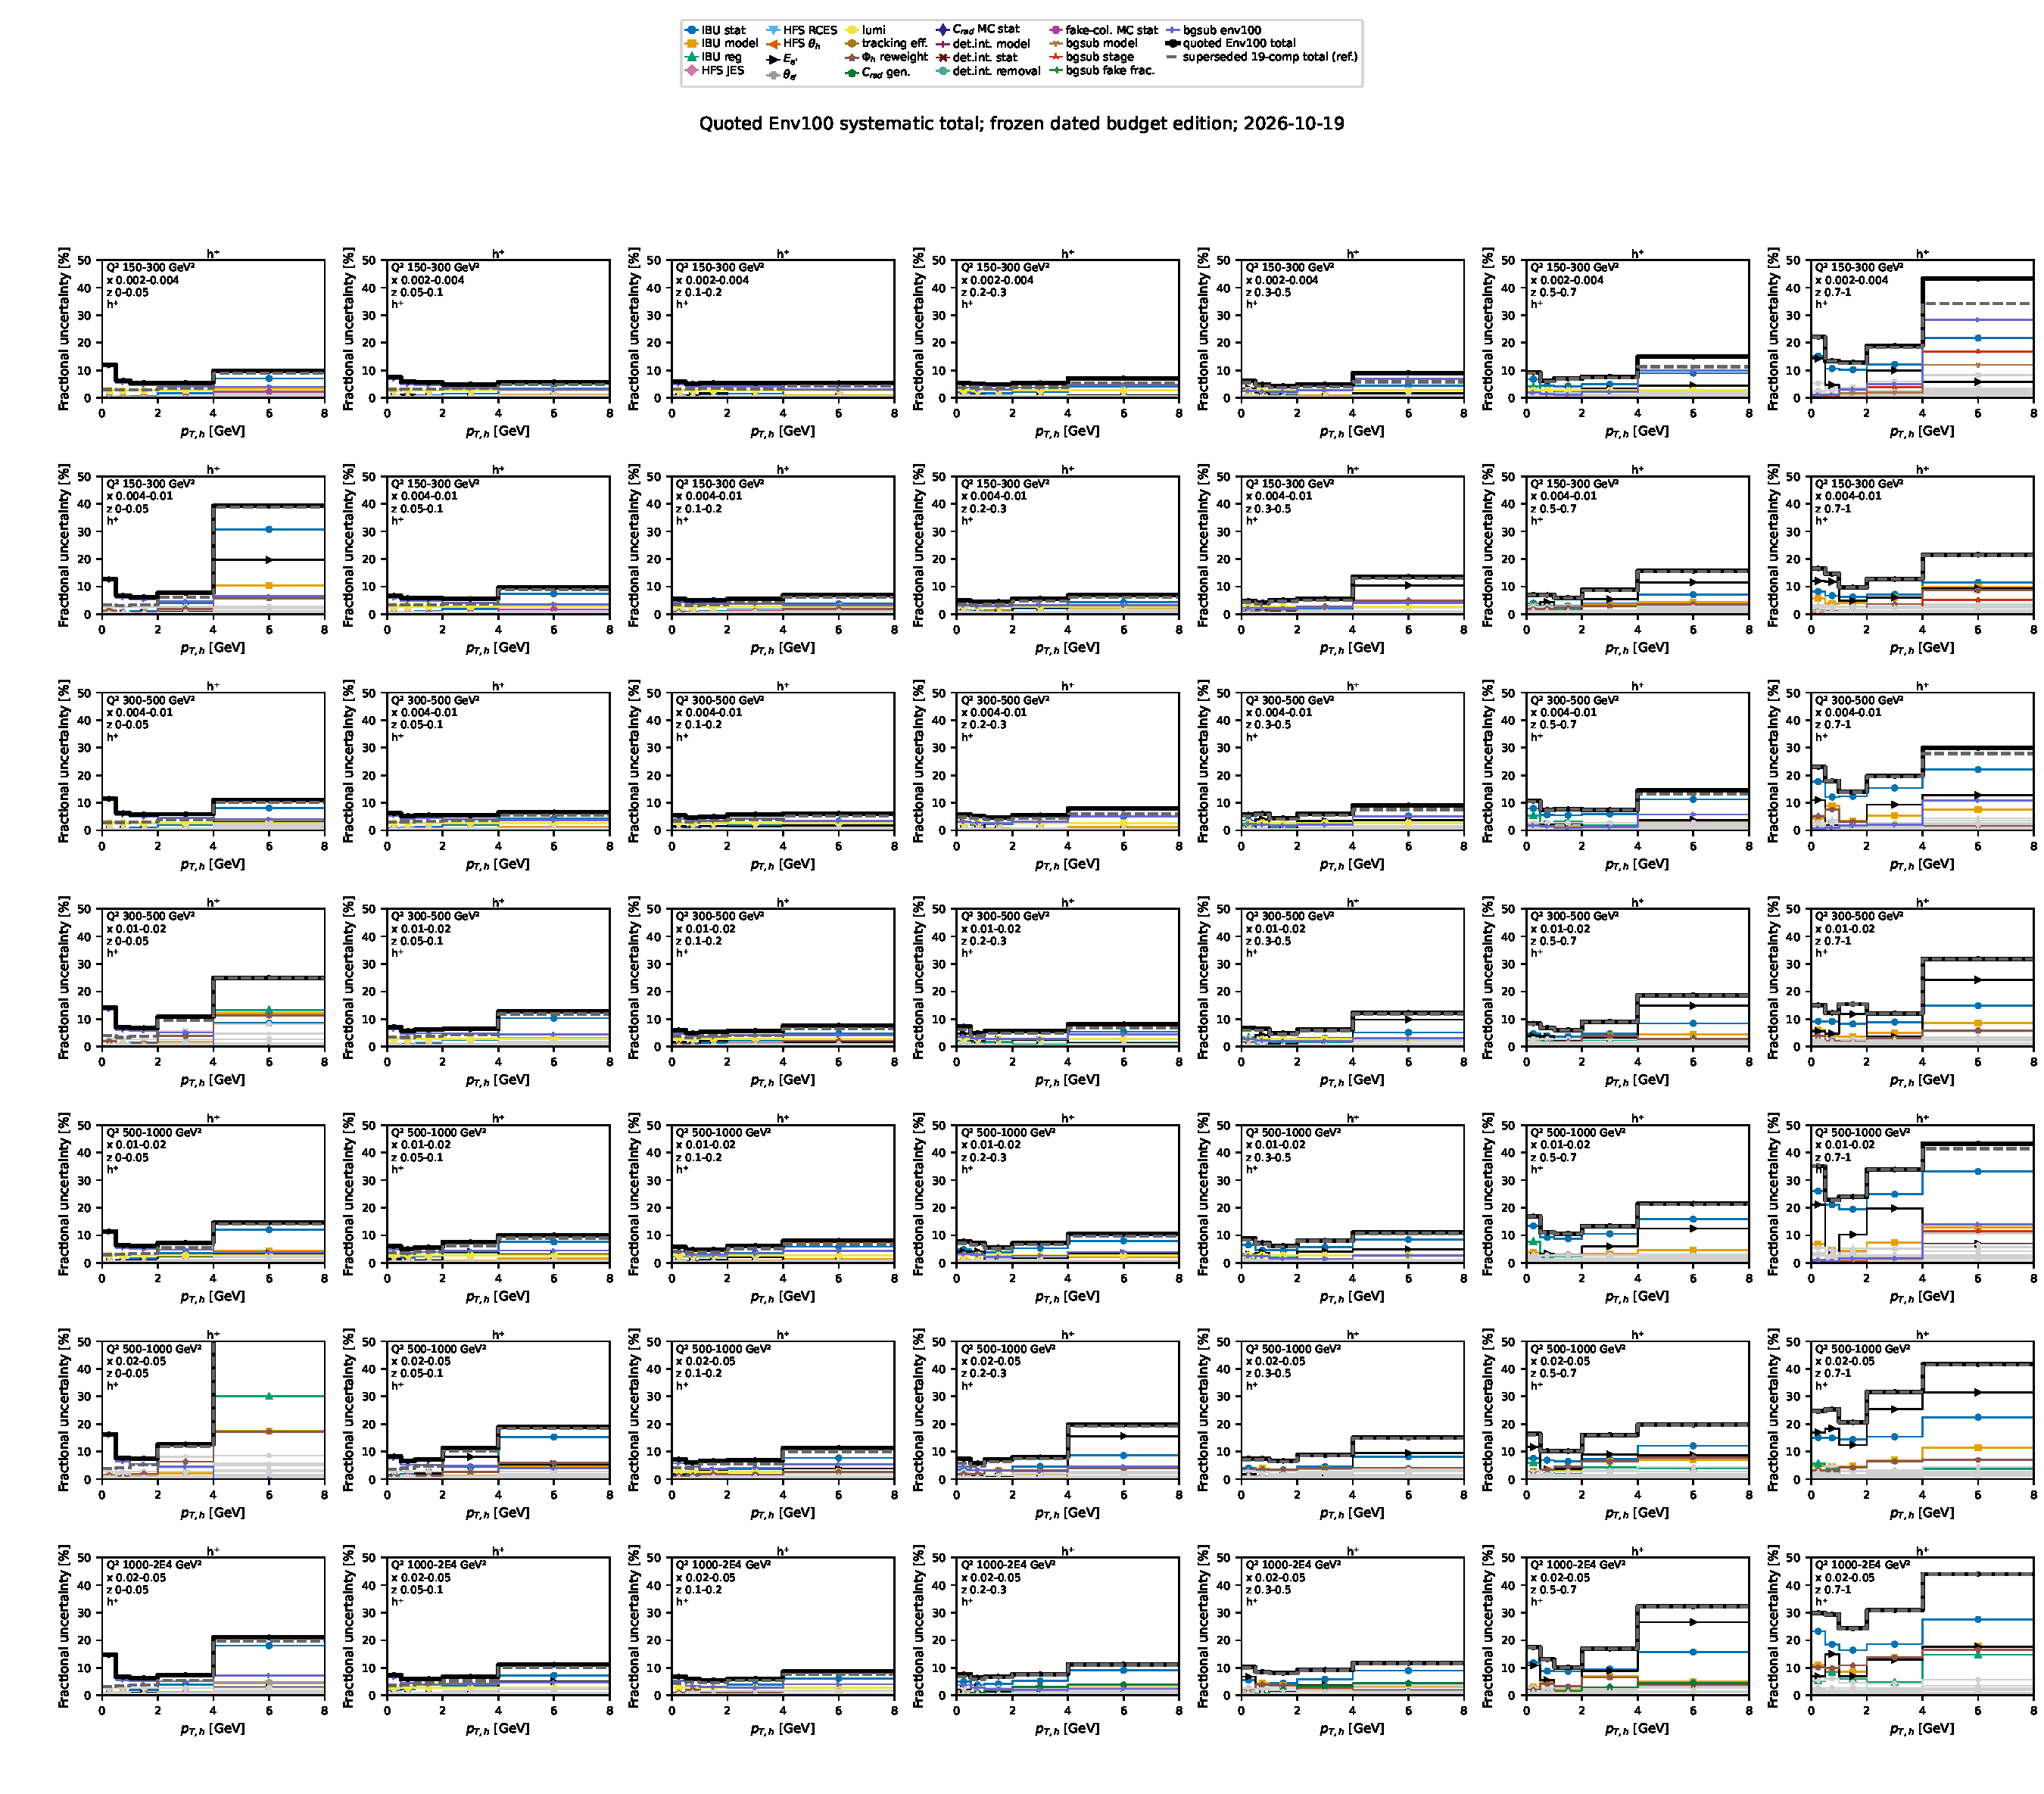
\includegraphics[width=0.98\textwidth,height=0.82\textheight,keepaspectratio]{figures/fig_syst_uncertainty_sources_hplus_env100_ylim050.pdf}
  \caption{Per-source fractional systematic uncertainties for $\hplus$ versus
  $\pTh$ on the frozen 2026-10-19 uncertainty basis, shown in percent units with a fixed
  0--50\% vertical range.}
  \label{fig:syst:sources-hplus-env100-midrange}
\end{figure}

\begin{figure}[p]
  \centering
  \begin{subfigure}[t]{0.98\textwidth}
    \centering
    \includegraphics[page=2,width=\textwidth,height=0.38\textheight,keepaspectratio]{figures/fig_syst_uncertainty_sources_hminus_env100_ylim100.pdf}
    \caption{Full 0--100\% range.}
  \end{subfigure}
  \par\medskip
  \begin{subfigure}[t]{0.98\textwidth}
    \centering
    \includegraphics[page=2,width=\textwidth,height=0.38\textheight,keepaspectratio]{figures/fig_syst_uncertainty_sources_hminus_env100_ylim015.pdf}
    \caption{0--15\% zoom.}
  \end{subfigure}
  \caption{Per-source fractional systematic uncertainties for $\hminus$ versus
  $\pTh$ on the frozen 2026-10-19 uncertainty basis, shown in percent units.}
  \label{fig:syst:sources-hminus-env100-fullrange}
\end{figure}

\begin{figure}[p]
  \centering
  \includegraphics[page=2,width=0.98\textwidth,height=0.82\textheight,keepaspectratio]{figures/fig_syst_uncertainty_sources_hminus_env100_ylim050.pdf}
  \caption{Per-source fractional systematic uncertainties for $\hminus$ versus
  $\pTh$ on the frozen 2026-10-19 uncertainty basis, shown in percent units with a fixed
  0--50\% vertical range.}
  \label{fig:syst:sources-hminus-env100-midrange}
\end{figure}

\subsection{Fractional Covariance Matrices}
\label{sec:syst:global-covariance}

The frozen 2026-10-19 uncertainty product provides fractional cross-section
covariance matrices on the 245 published bins per charge.  The matrices are
constructed for the current observable basis, with the near-electron cone
selection, the electron, V0, and low-$\Qsq$ backgrounds subtracted from the
data before unfolding, and the iterative Bayesian unfolding result taken on
the subtracted data vector.  They
encode the 20 active terms of the current budget: \texttt{ibu\_stat\_rel}
and 19 systematic terms.  The retired \texttt{bgsub\_stat\_rel} column is not
included.

The correlation model is deliberately limited to validated declarations.
The luminosity and \texttt{bgsub\_env100\_rel} terms are fully correlated
across all bins and between charges.  All other components are represented
as bin-diagonal because no validated inter-bin correlation model is available
for them in this edition.  Consequently, the cross-charge covariance contains
only the luminosity and background-envelope rank-one terms; the IBU
statistical term is
stored separately as a diagonal fractional covariance.  The diagonal of the
combined covariance reproduces \texttt{total\_with\_env100\_rel}$^2$, with
maximum relative deviations of $5.431899438732146\times10^{-15}$ for
$\hplus$ and $6.403330938130179\times10^{-15}$ for $\hminus$.

The matrices are symmetric and positive definite in each charge block: the
minimum fractional eigenvalues are $7.681667696346608\times10^{-5}$ for
$\hplus$ and $8.165371868314269\times10^{-5}$ for $\hminus$.  The
cross-charge block is symmetric.  These matrices provide the declared
fractional-covariance model only; they do not supply a new response-MC
statistical covariance or a correlation model for the bin-diagonal
components.  Any use must state the Born-versus-raw level of the nominal
cross section used to convert fractional covariance to cross-section units.

The product is retained at
\path{/data/dust/group/h1/klesthen/BaryonAsym/H1ChargedSidis_HighQ2/output_v6/central/data_release/systematics_bgsub_env100_21comp_2026-10-19/covariance/}.
It contains the per-charge and cross-charge fractional systematic covariance
matrices, the separately stored IBU-statistical matrices, a total-correlation
rendering, and the gate record.  The gate record and release status report
all covariance/correlation checks as passed.  The package was constructed on
the superseded central values and is pending re-basing to the OPT-A nominal
(Sec.~\ref{sec:syst:budget-regeneration}); its diagonals also carry the
conservative detector-interaction double count of the frozen total.

\subsection{Detector and Track-Selection Robustness Cross-Checks}
\label{sec:syst:cut-variations}

In addition to the systematic components included in the nominal budget, several
detector and track-selection variants have been performed as robustness checks
rather than central results. Ideally, the measurement would be insensitive to
small changes in detector-level cuts. We study the effect of varying the $E-p_z$
cut, the minimum lab-frame $p_T$, the $\eta$ cut, and the cut on the distance of
closest approach, generating a new migration matrix with these reconstructed-level
cuts and then repeating the IBU unfolding procedure on the data. The results are
shown as the ratio of the unfolded cross section with the nominal cut to the
measured cross section with the varied cut for all bins in
\cref{fig:syst:cutvar-empz25,fig:syst:cutvar-labpt,fig:syst:cutvar-eta,fig:syst:cutvar-dca1,fig:syst:cutvar-dca3}. The uncertainties on the points in these figures show the model, statistical, and regularization uncertainties of the IBU unfolding.
These variants were produced before the coherent-prior re-release and the
subsequent detector-interaction and cone-baseline promotions, on an earlier
release lineage; they are retained as robustness checks of the cut scheme and
have not been repeated on the current cone-based release.

The loosening or tightening of the DCA cut is observed to have essentially no impact on the result. The lab $p_T$ cut has a 3-4\% effect on the lowest $\pTh$ bins, with one bin (with huge statistical uncertainties) exhibiting a 10\% shift. The lab $\eta$ cut has the most significant impact, due to the fact that it removes a much larger number of particles. A few bins are reduced to having low statistics after imposing the $|\eta|<1.4$ cut, so large fluctuations in the unfolded data in these bins can be expected. As before, these bins generally already have a large systematic and statistical uncertainty. Even in the worse case, all bins lie within 2 sigma of the unvaried results.


\begin{table}[h]
\centering
\small
\begin{tabular}{p{2.5cm}p{4.7cm}p{2.1cm}p{2.1cm}p{2.1cm}}
\toprule
Study & Reco-level change  & Ratio min & Ratio median & Ratio max\\
\midrule
Lab-$p_T$ & $P_{T,\mathrm{lab}}^{\min}:0.15\rightarrow0.10~\GeV$  & 0.962 & 1.000 & 1.111 \\
$|\eta|$ & $|\eta_{\mathrm{lab}}|:1.6\rightarrow1.4$ & 0.562 & 1.001 & 1.296 \\
DCA$<1$ & $\mathrm{DCA}'\sin\theta < 1.0\,\mathrm{cm}$  & 0.990 & 1.000 & 1.043 \\
DCA$<3$ & $\mathrm{DCA}'\sin\theta < 3.0\,\mathrm{cm}$ & 0.999 & 1.000 & 1.000 \\
\bottomrule
\end{tabular}
\caption{Detector and track-selection robustness checks rather than central results, summarizing the results shown in \cref{fig:syst:cutvar-labpt,fig:syst:cutvar-eta,fig:syst:cutvar-dca1,fig:syst:cutvar-dca3}.}
\label{tab:syst:cut-variation-summary}
\end{table}

Each variant satisfies the same basic validation contract as the nominal
analysis products: 490 IBU rows, $N_{B,G}=245$, $N_{B,R}=490$, finite central
values, and no negative cross sections.  The lab-$p_T$ and $|\eta|$ variants and
the two DCA variants each have complete migration-QA plot bundles with 42 PDF
and 42 PNG outputs.  The DCA variants were additionally checked to have 490/490
finite IBU rows and zero missing ratio rows.

\begin{figure}[p]
  \centering
  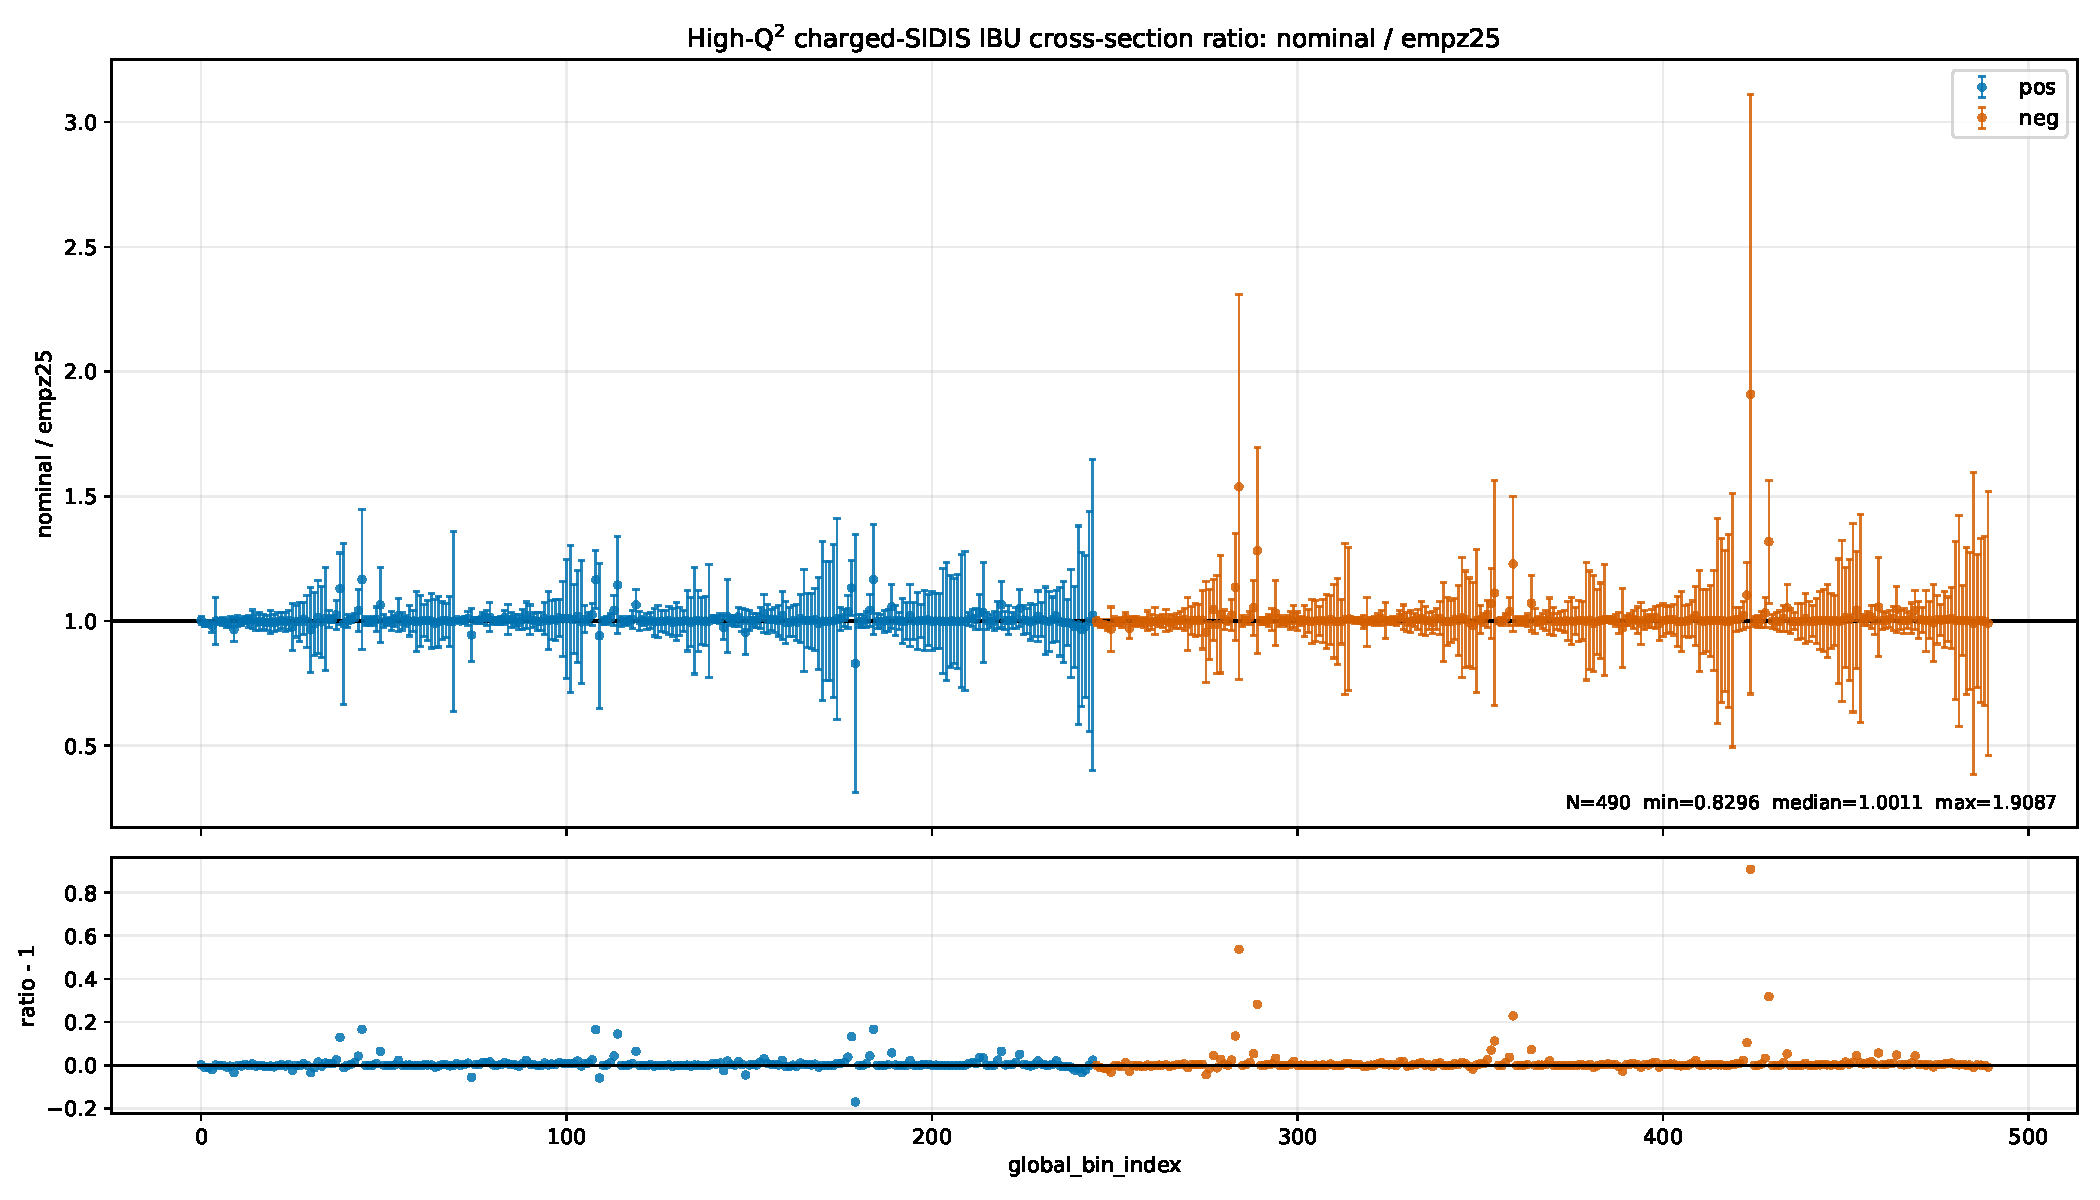
\includegraphics[width=0.95\textwidth]{figures/fig_cutvar_empz25_ratio.pdf}
  \caption{Global bin ratio of the unfolded cross sections for the reconstructed
  \mbox{$E-p_z>35\,\mathrm{GeV}\to E-p_z>25\,\mathrm{GeV}$} threshold variation.}
  \label{fig:syst:cutvar-empz25}
\end{figure}

\begin{figure}[p]
  \centering
  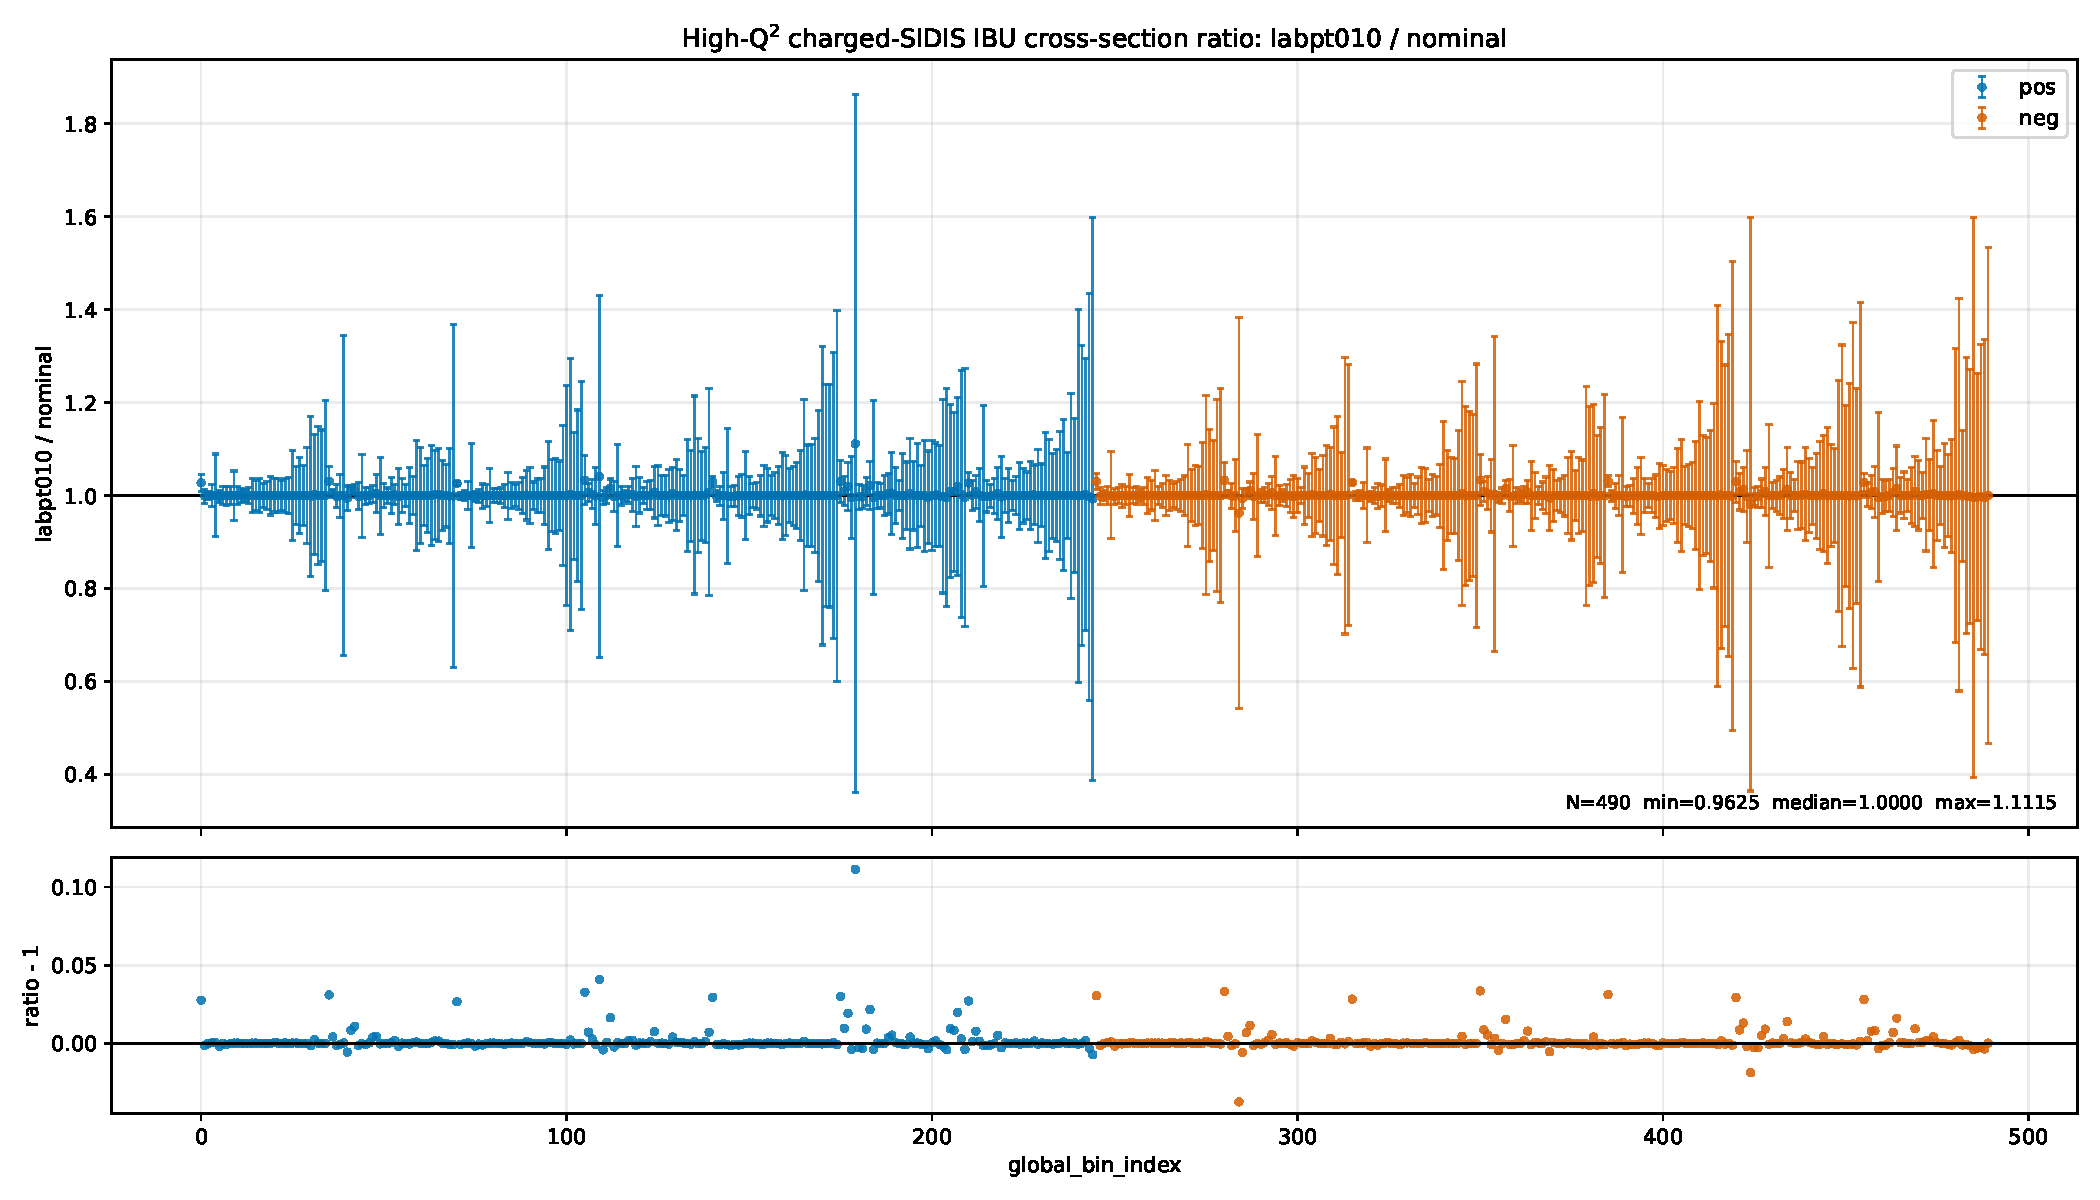
\includegraphics[width=0.95\textwidth]{figures/fig_cutvar_labpt010_ratio.pdf}
  \caption{Global bin ratio of the unfolded cross sections for the reconstructed lab-frame \mbox{\(p_T<0.15\,\mathrm{GeV}\to p_T<0.10\,\mathrm{GeV}\)}threshold
  variation.}
  \label{fig:syst:cutvar-labpt}
\end{figure}

\begin{figure}[p]
  \centering
  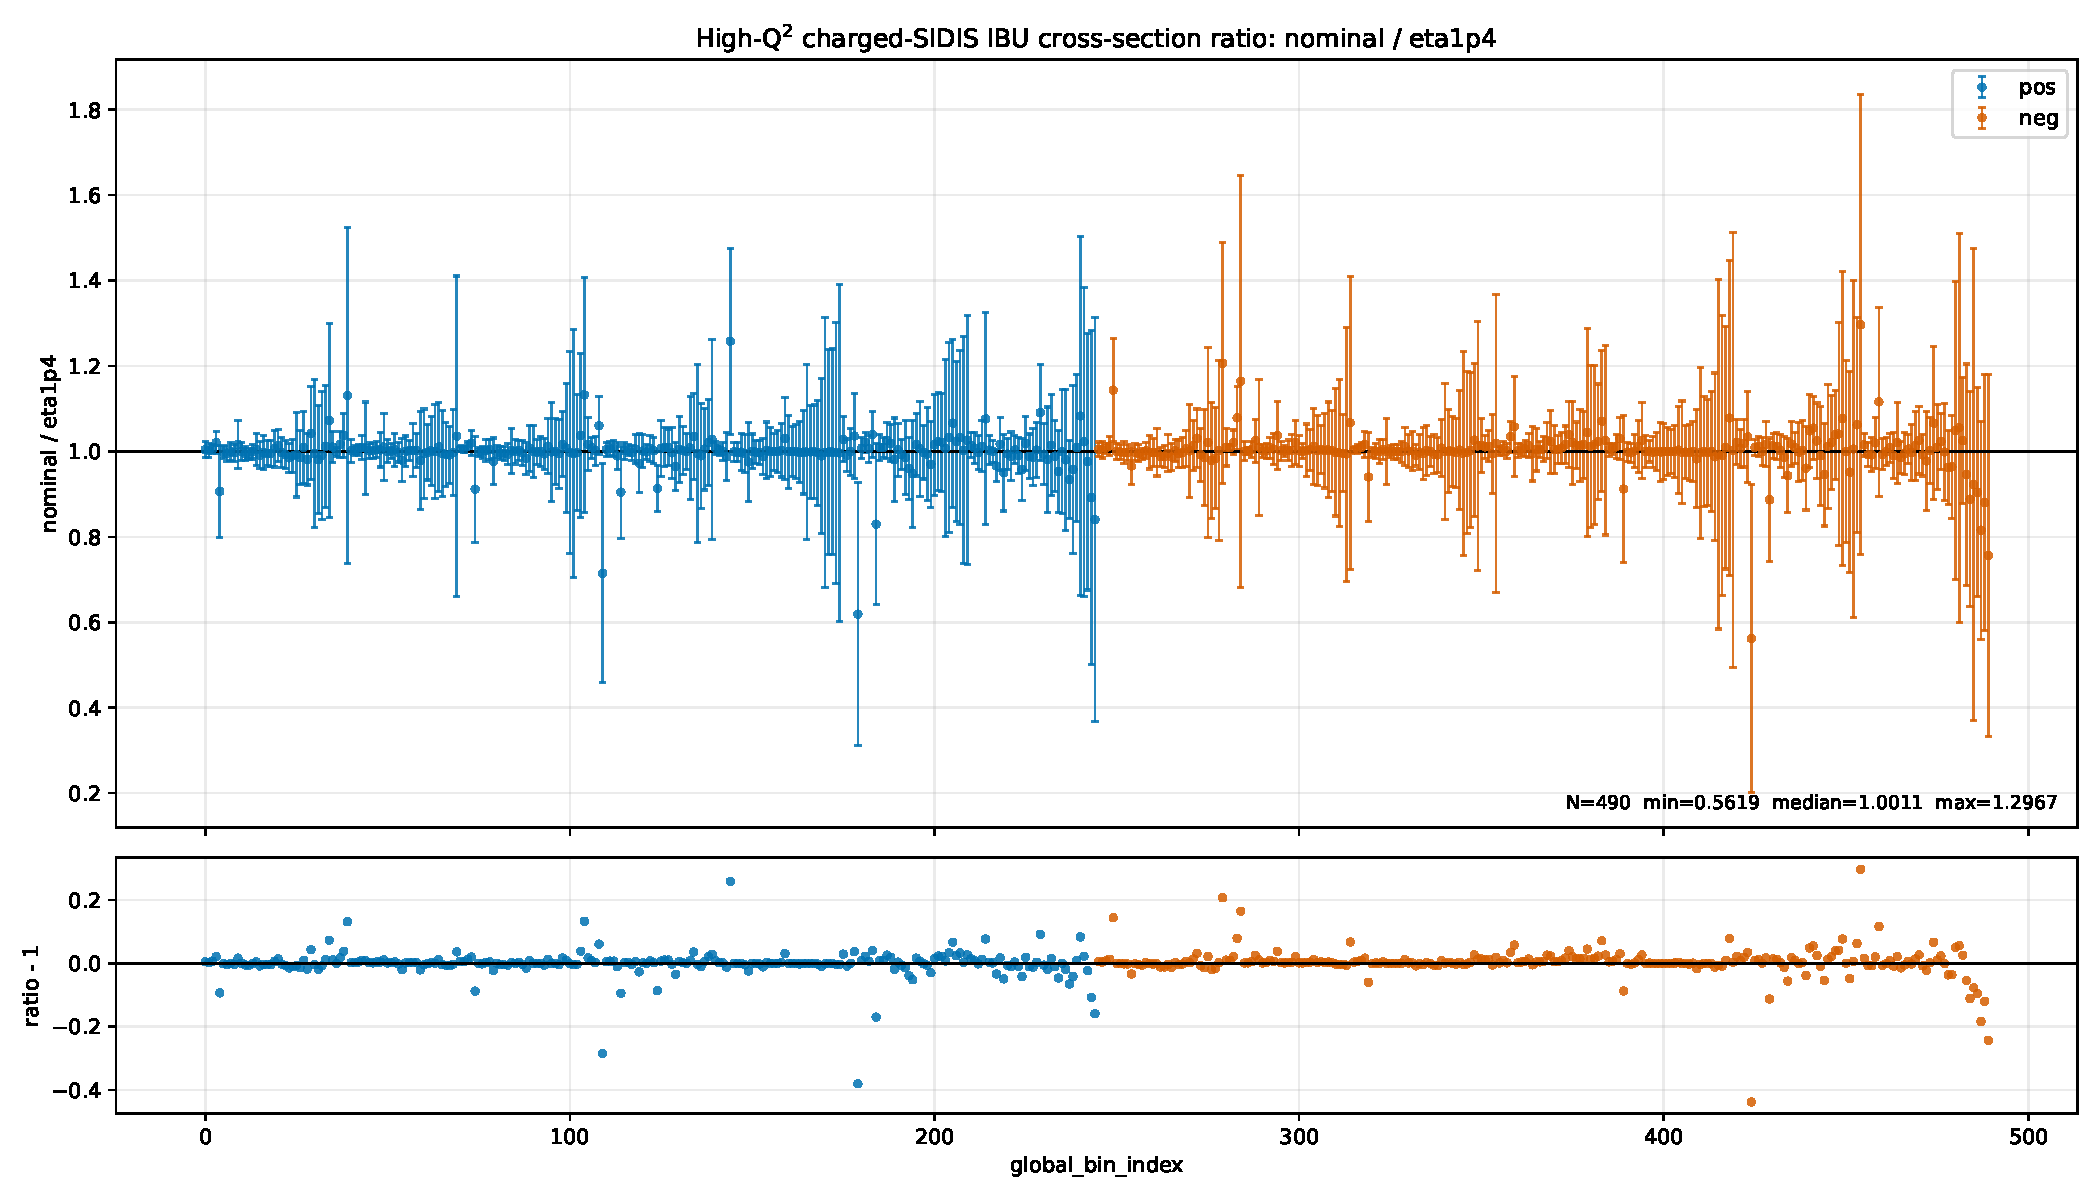
\includegraphics[width=0.95\textwidth]{figures/fig_cutvar_eta1p4_ratio.pdf}
  \caption{Global bin ratio of the unfolded cross sections for the reconstructed lab-frame \mbox{$|\eta|<1.6\to|\eta|<1.4$} threshold
  variation.}
  \label{fig:syst:cutvar-eta}
\end{figure}

\begin{figure}[p]
  \centering
  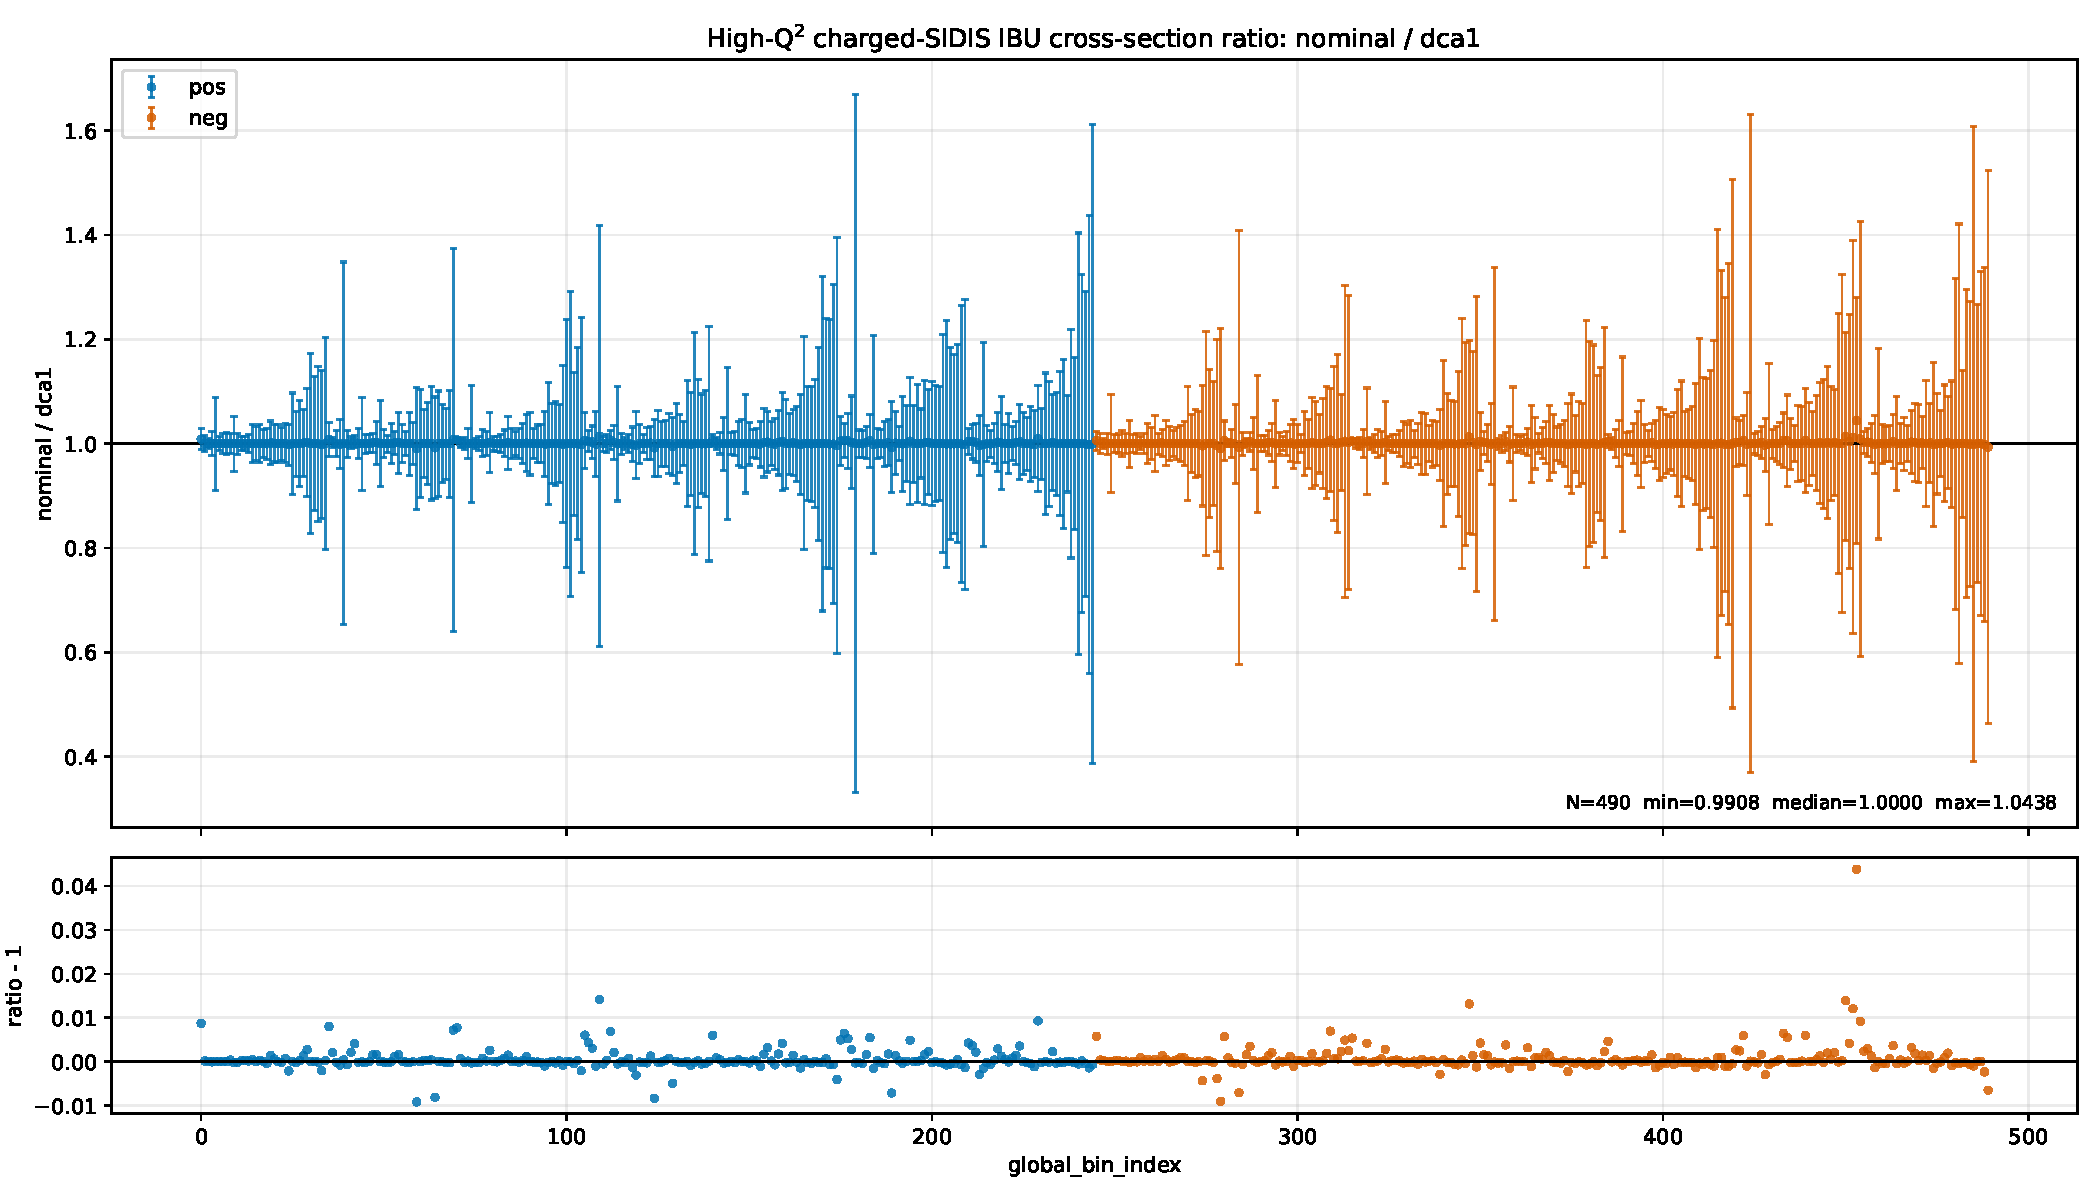
\includegraphics[width=0.95\textwidth]{figures/fig_cutvar_dca1_ratio.pdf}
  \caption{Global bin ratio of the unfolded cross sections for the reconstructed
  \mbox{$\mathrm{DCA}'\sin\theta < 2\,\mathrm{cm} \to \mathrm{DCA}'\sin\theta < 1\,\mathrm{cm}$}
  threshold variation.}
  \label{fig:syst:cutvar-dca1}
\end{figure}

\begin{figure}[p]
  \centering
  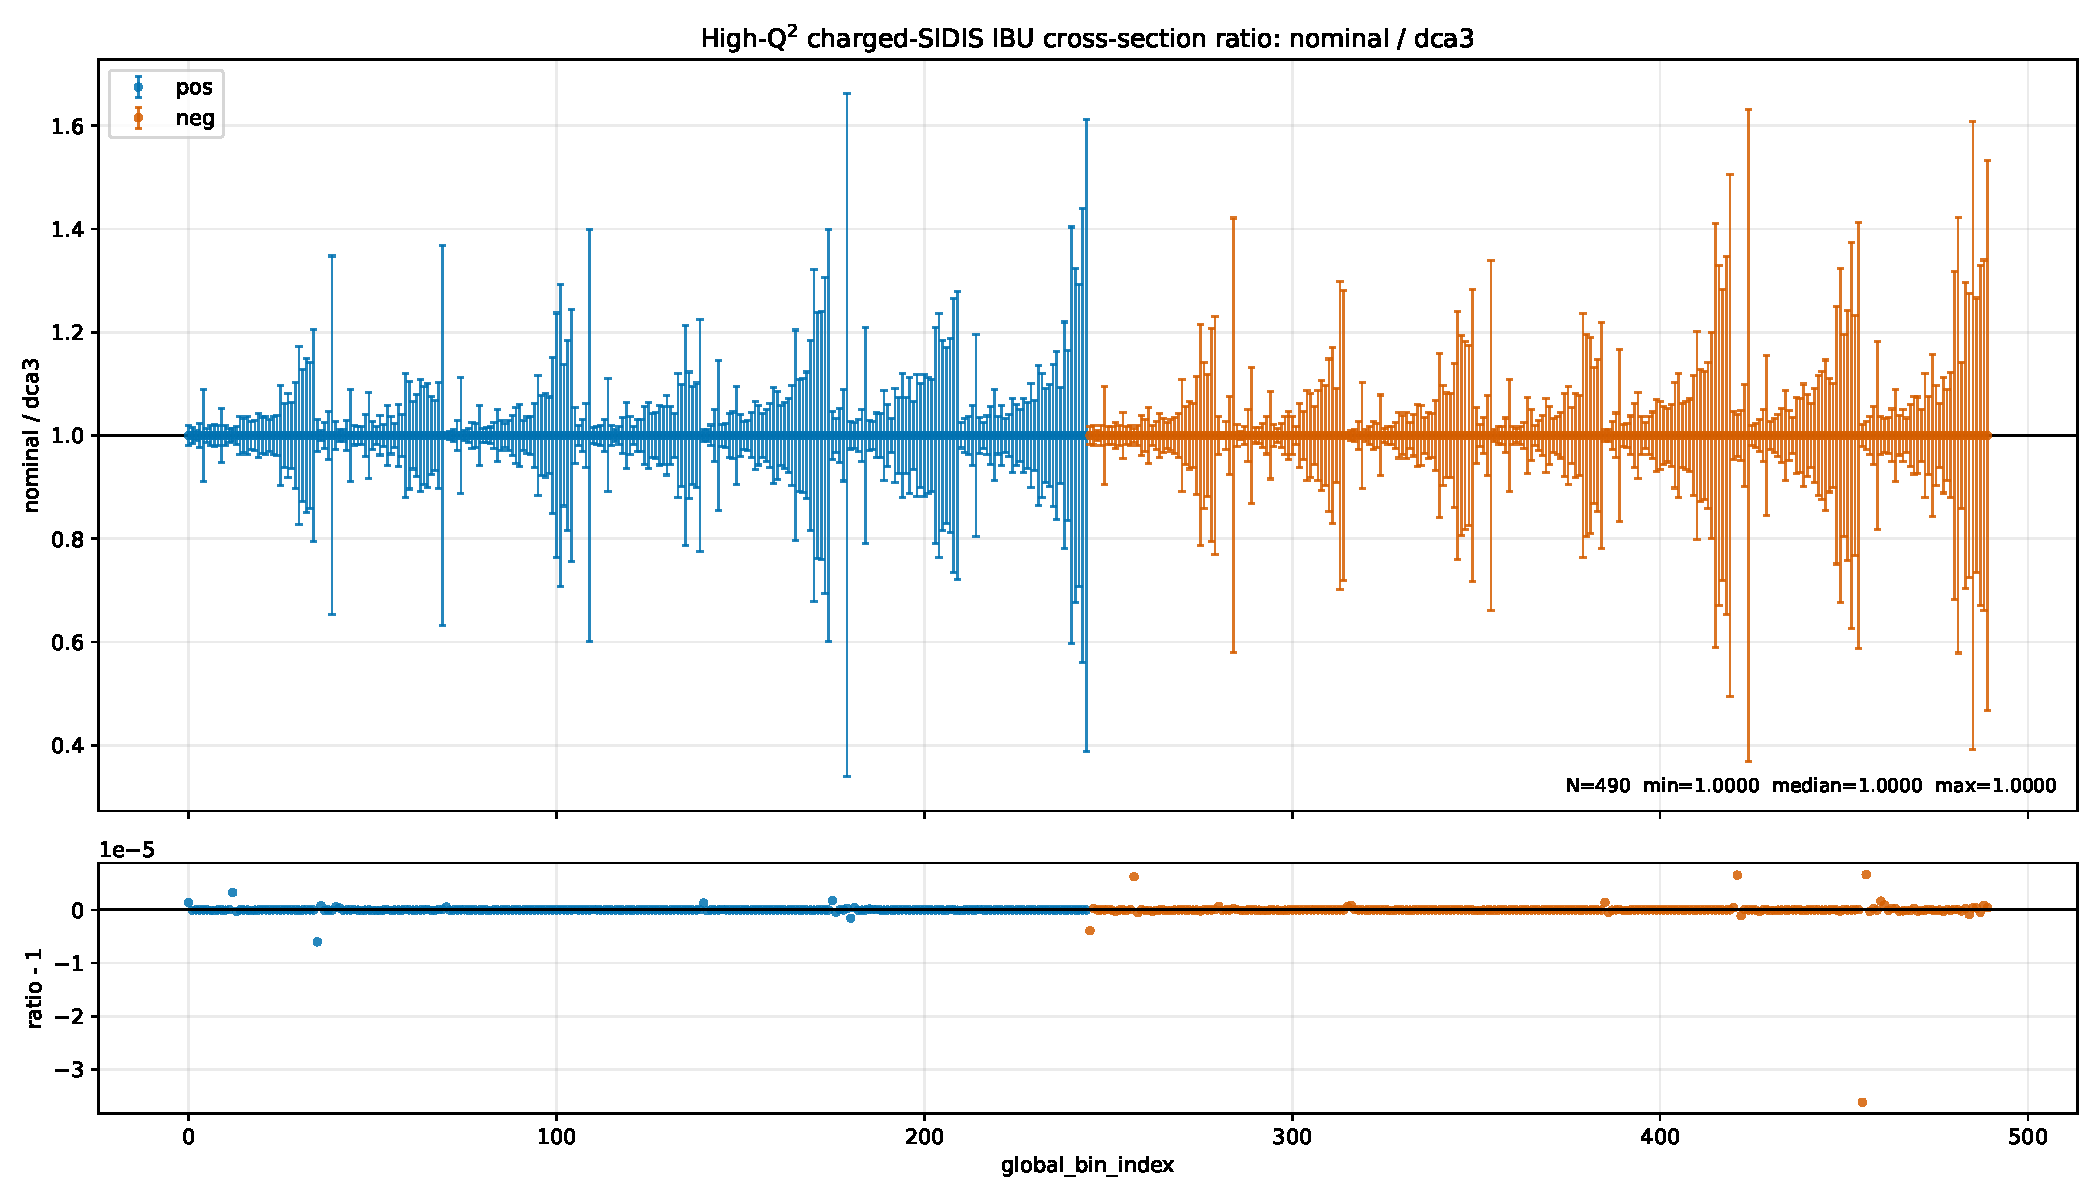
\includegraphics[width=0.95\textwidth]{figures/fig_cutvar_dca3_ratio.pdf}
  \caption{Global bin ratio of the unfolded cross sections for the reconstructed
  \mbox{$\mathrm{DCA}'\sin\theta < 2\,\mathrm{cm} \to \mathrm{DCA}'\sin\theta < 3\,\mathrm{cm}$}
  threshold variation.}
  \label{fig:syst:cutvar-dca3}
\end{figure}

\subsection{Near-Electron Opening-Angle Diagnostic}
\label{sec:syst:near-electron-alpha}
The previous H1 results (Refs.~\cite{H1:2013qsm,H1:2020zpd}) use a track--scattered-electron angle requirement larger than 0.2 rad to suppress anomalous tracks appearing near the scattered electron. These tracks could arise from photon conversions of final-state radiation (at the vertex or in detector material) off the electron, or tracks from the scattered electron which are mis-identified as not belonging to the scattered electron~\cite{Grebenyuk:2012thesis}. In the latter case, it would be expected that the track energy would be relatively close to the scattered electron energy measured in the calorimeter. The reconstructed momentum of the tracks very near to the scattered electron does not correlate strongly to the scattered electron energy, supporting the photon conversion hypothesis over the electron track mis-ID hypothesis.

Since the cone-baseline promotion of 2026-10-13, the
$\alpha\ge0.2~\mathrm{rad}$ laboratory-frame cone on the reconstructed legs is
part of the central selection basis rather than a diagnostic variant.  The
cone is applied after the electron and V0 truth vetoes and before the
matched-fake classification; cone-rejected matched legs flow to the miss row
of the response, and the coherent prior is computed from the response variant
that carries both the cone selection and the detector-interaction correction.
The diagnostic ratios in
Table~\ref{tab:syst:alpha-veto-integrated} were produced before that
promotion and are retained as motivation for the cone requirement.

\begin{table}[h]
\centering
\small
\begin{tabular}{p{4.4cm}p{2cm}p{2cm}}
\toprule
Quantity for $\alpha<0.2$ & RAPGAP & DJANGOH \\
\midrule
Integrated true $\pi/K/p$ loss & 0.106\% & 0.114\% \\
Residual $e^{\pm}$ / true $\pi/K/p$
  & $4.38\%$
  & $4.39\%$ \\
%V0-daughter / true $\pi/K/p$
%  & $3.90\%$
%  & $3.88\%$ \\
\bottomrule
\end{tabular}
\caption{Integrated MC-only diagnostic ratios for the near-electron opening-angle
study.}
\label{tab:syst:alpha-veto-integrated}
\end{table}
